\documentclass{article}
\usepackage{fullpage,palatino,mathpazo,amsmath,amssymb,url}
\usepackage{url,amsmath,amssymb,subfigure,boxedminipage,shadow}
\usepackage[pdftex]{graphicx,color}
\usepackage{listings,tabularx,booktabs,hyperref}
%\usepackage{hevea}
\graphicspath{{Figures/}}

\newcolumntype{C}[1]{>{\centering\arraybackslash}p{#1}} % centering column type with fixed width
\newcolumntype{R}[1]{>{\raggedleft\arraybackslash}p{#1}} % right aligned column type with fixed width
\newcolumntype{L}[1]{>{\raggedright\arraybackslash}p{#1}} % left aligned column type with fixed width

\newcounter{colend}
\newcounter{maxcol}
\newcounter{mincol}

\newcounter{facnt}
\newcounter{hacnt}
\newcounter{dotcnt}

% usage: \begin{dotdiag}{colwidth}
\newenvironment{dotdiag}[1]{%
  \setcounter{maxcol}{#1}
  \setcounter{facnt}{0}
  \setcounter{hacnt}{0}
  \setcounter{dotcnt}{0}
  \setcounter{mincol}{0}
  \begin{tikzpicture}[scale=0.5]
}{\end{tikzpicture}}

% usage: \drawdotcol[row]{col}{height}
\newcommand*\drawdotcol[3][0]{
  \setcounter{colend}{#3}
  \ifnum \value{colend} > 0 {   
    \addtocounter{colend}{-1}%
    \addtocounter{colend}{#1}%
    \foreach \t in {#1,...,\value{colend}}{
      \draw[fill=black] (\value{maxcol}-#2,\t) circle (0.2);
      \addtocounter{dotcnt}{1}
    }
  }
  \else {% still draw a transparent circle for figure alignment 
    \draw[opacity=0,fill=black] (\value{maxcol}-#2,0) circle (0.2);
  }
  \fi
}

% usage: \drawtrunccol{col}{height} (to draw truncated bit heaps)
\newcommand*\drawtrunccol[3][0]{ 
  \setcounter{colend}{#3}
  \addtocounter{colend}{-1}%
  \addtocounter{colend}{#1}%

  \ifnum #3 > 0   
    \foreach \t in {#1,...,\value{colend}}{
      \draw[black!50, fill=white] (\value{maxcol}-#2,\t) circle (0.2);
  	  \addtocounter{dotcnt}{1}
    }
  \fi
}

% usage: \drawdotrow[row]{col}{width}
\newcommand*\drawdotrow[3][0]{
  \setcounter{colend}{#3}
  \addtocounter{colend}{-1}%
  \addtocounter{colend}{#1}%

  \foreach \t in {#1,...,\value{colend}}{
    \draw[fill=black] (\value{maxcol}-\t,#2) circle (0.2);
  	\addtocounter{dotcnt}{1}
  }
}

% usage: \drawtruncrow[row]{col}{width}
\newcommand*\drawtruncrow[3][0]{
  \setcounter{colend}{#3}
  \addtocounter{colend}{-1}%
  \addtocounter{colend}{#1}%

  \foreach \t in {#1,...,\value{colend}}{
    \draw[black!50,fill=white] (\value{maxcol}-\t,#2) circle (0.2);
  	\addtocounter{dotcnt}{1}
  }
}

% usage: \drawdotone{col}{row}
\newcommand*\drawdotone[2]{
  \node at (\value{maxcol}-#1,#2) {\footnotesize \textcircled{\scalebox{0.7}{1}}};

%  \addtocounter{dotcnt}{1}
}

% usage: \drawdottext{col}{row}
\newcommand*\drawdottext[3]{
  \node at (\value{maxcol}-#1,#2) {\textbf{#3}};
%  \addtocounter{dotcnt}{1}
}

% usage: \drawdot[color]{col}{row}
\newcommand*\drawdot[3][black]{
	\draw[fill=#1] (\value{maxcol}-#2,#3) circle (0.2);
	\addtocounter{dotcnt}{1}
}

% usage: \drawhalf[color]{col}{row}
\newcommand*\drawhalf[3][magenta]{
  \pgfsetcornersarced{\pgfpoint{2.5mm}{2.5mm}}
  \draw[fill=#1!50,opacity=0.75] (\value{maxcol}-#2-0.5,#3-0.5) rectangle +(1,2);
  \addtocounter{hacnt}{1}
  \pgfsetcornersarced{\pgfpointorigin}
}

% usage: \drawfull[color]{col}{row}
\newcommand*\drawfull[3][cyan]{
  \pgfsetcornersarced{\pgfpoint{2.5mm}{2.5mm}}
  \draw[fill=#1!50,opacity=0.75] (\value{maxcol}-#2-0.5,#3-0.5) rectangle +(1,3);
  \addtocounter{facnt}{1}
  \pgfsetcornersarced{\pgfpointorigin}
}

% usage: \drawhalfres[color]{col}{row}
\newcommand*\drawhalfres[2]{
%no line markers:
%  \draw (\value{maxcol}-#1-1,#2) -- +(1,0);
%vertical line markers:
%  \draw (\value{maxcol}-#1-1,#2) -- +(0.5,0) -- +(0.5,0.125) -- +(0.5,-0.125) -- +(0.5,0) -- +(1,0);
%diagonal line markers:
  \draw (\value{maxcol}-#1-1,#2) -- +(0.5,0) -- +(0.5-0.125,-0.125) -- +(0.5+0.125,0.125) -- +(0.5,0) -- +(1,0);
}

% usage: \drawfullres[color]{col}{row}
\newcommand*\drawfullres[2]{
  \draw (\value{maxcol}-#1-1,#2) -- +(1,0);
}

% usage: \drawcpa[col]{width}
\newcommand*\drawcpa[2][0]{
  \pgfsetcornersarced{\pgfpoint{2.5mm}{2.5mm}}
  \draw[fill=blue!50,opacity=0.75] (\value{maxcol}-#2-#1+0.5,-0.5) rectangle +(#2,2);
%  \draw[fill=blue!50,opacity=0.75] (\value{maxcol}-#2-#1+0.5,-0.5) -- ++(#2,0) -- ++(0,3) -- ++(-1,0) --  ++(0,-1) -- ++(-#2+1,0) -- cycle;
  \pgfsetcornersarced{\pgfpointorigin}
}

% usage: \drawcpawithcarry[col]{width}
\newcommand*\drawcpawithcarry[2][0]{
  \pgfsetcornersarced{\pgfpoint{2.5mm}{2.5mm}}
%  \draw[fill=blue!50,opacity=0.75] (\value{maxcol}-#2-#1+0.5,-0.5) rectangle +(#2,2);
  \draw[fill=blue!50,opacity=0.75] (\value{maxcol}-#2-#1+0.5,-0.5) -- ++(#2,0) -- ++(0,3) -- ++(-1,0) --  ++(0,-1) -- ++(-#2+1,0) -- cycle;
  \pgfsetcornersarced{\pgfpointorigin}
}

% usage: \drawlegend[row]
\newcommand*\drawlegend[1][0]{
  \draw (\value{maxcol}-1.5,#1+1) node {$\leftarrow$ column};
  \foreach \t in {\themincol,...,\themaxcol}{
	\draw (\value{maxcol}-\t,#1) node {\t};
  }
}

% usage: \drawline[row]
\newcommand*\drawline[1][0]{
  \draw[thick] (0,-#1-1) -- ++(\value{maxcol}+1,0);
}


\usepackage{tikz}
\newcommand{\operator}{ \verb!Operator! }

\title{\scalebox{0.3}{\mbox{\input{../Figures/flopocoLogo.pdf_t}}}\\
FloPoCo \input{../../VERSION} developer manual
}

\author{Florent de Dinechin+}

\graphicspath{{../Figures/}}
\pagestyle{empty}

\begin{document} 
\sloppy



\maketitle


Welcome to new developers! 

The purpose of this document is to help you use FloPoCo in your own
project (section~\ref{sec:getting-started} to \ref{sec:data-types}), and to show you how to design your own pipelined operator
using the FloPoCo framework (sections~\ref{sec:tutorial} and \ref{sec:test-bench-gener}). 

\tableofcontents

\section{Getting started with FloPoCo\label{sec:getting-started}}


\subsection{Getting the source and compiling using CMake}

It is strongly advised that you work with the git version of the source, which can be obtained by following the instructions on
\url{http://flopoco.org/flopoco_installation.html}. If you wish to distribute your work with FloPoCo, contact us.

If you are unfamiliar with the CMake system, there is little to learn,
really. When adding .hpp and .cpp files to the project, you will need
to edit \texttt{src/SourceFileList.txt}. It is probably going to be straightforward,
just do some imitation of what is already there. Anyway \texttt{cmake} is well
documented. The web page of the CMake project is \url{http://www.cmake.org/}.

\subsection{Linking against FloPoCo\label{sec:linking}}
All the operators provided by the FloPoCo command line are available
programmatically in libFloPoCo. A minimal example of using this
library is provided in \texttt{src/main\_minimal.cpp}.

It is best to use an operator through its factory. The file \texttt{src/main.cpp} is the source of the FloPoCo command
line, and as such uses most operators: looking at it is the quickest
way to look for the interface of a given operator.

The other way is, of course, to look at the corresponding \texttt{hpp}
file -- they are all included by \texttt{src/Operator.hpp}. Some
operators offer more constructors (richer interface options) than what
is used in \texttt{src/main.cpp}.


There should be a Doxygen documentation of FloPoCo.

\subsection{Overview of FloPoCo code organization}

The core of FloPoCo is the \texttt{Operator} class. 
Operator is a virtual class from which all FloPoCo operators inherit. 

The FloPoCo source includes a dummy operator, \texttt{TutorialOperator}, for you to play with. 
Feel free to experiment within this one. 
By default it is compiled but unplugged. To plug it back, just comment the corresponding line in main.cpp.

A good way to design a new operator is to imitate a simple one. We suggest
%\texttt{IntAdder} or 
\texttt{Shifter} for simple integer operators, and \texttt{FPAddSinglePath}
for a complex operator with several sub-components.
% An example of assembling several FP operators in a larger pipeline is \texttt{Collision}.

Meanwhile, browse through \texttt{Operator.hpp}. It has become quite bloated, showing
the history of the project. Try not to use methods flagged as
deprecated, as they will be removed in the future. Hopefully.%  Instead, use the
% automatic pipeline framework is described in Section~\ref{sec:pme}
% below.

Another important class hierarchy in FloPoCo is \texttt{Target}, which
defines the architecture of the target FPGA. It currently has several sub-classes,
including \texttt{Virtex} and \texttt{Stratix} targets. You may want to
add a new target, the best way to do so is by imitation. Please
consider contributing it to the project.

The command-line parser is in \texttt{UserInterface} but in principle you won't have to edit it.
It takes information from each operator's documentation strings defined in their \texttt{registerFactory()} methods. 
Again, we hope that you can design the interface to your operator by imitation of existing ones.

\subsection{Adding a new operator to FloPoCo}
To add a new operator to FloPoCo, you need to 
\begin{itemize}
\item write its \texttt{.cpp} and \texttt{.hpp} (we suggest you start with a copy of  \texttt{TutorialOperator}, which is an almost empty skeleton);
\item add it to \texttt{src/SourceFileList.txt} so that it gets compiled;
\item add it to \texttt{src/Factories/Interfaced.txt} if you want it to appear in the command-line interface.
\end{itemize}

That should be all. The rest is arithmetic!

And do not hesitate to contact us: \texttt{Florent.de.Dinechin@insa-lyon.fr}.

\begin{center}
%  \begin{latexonly}
  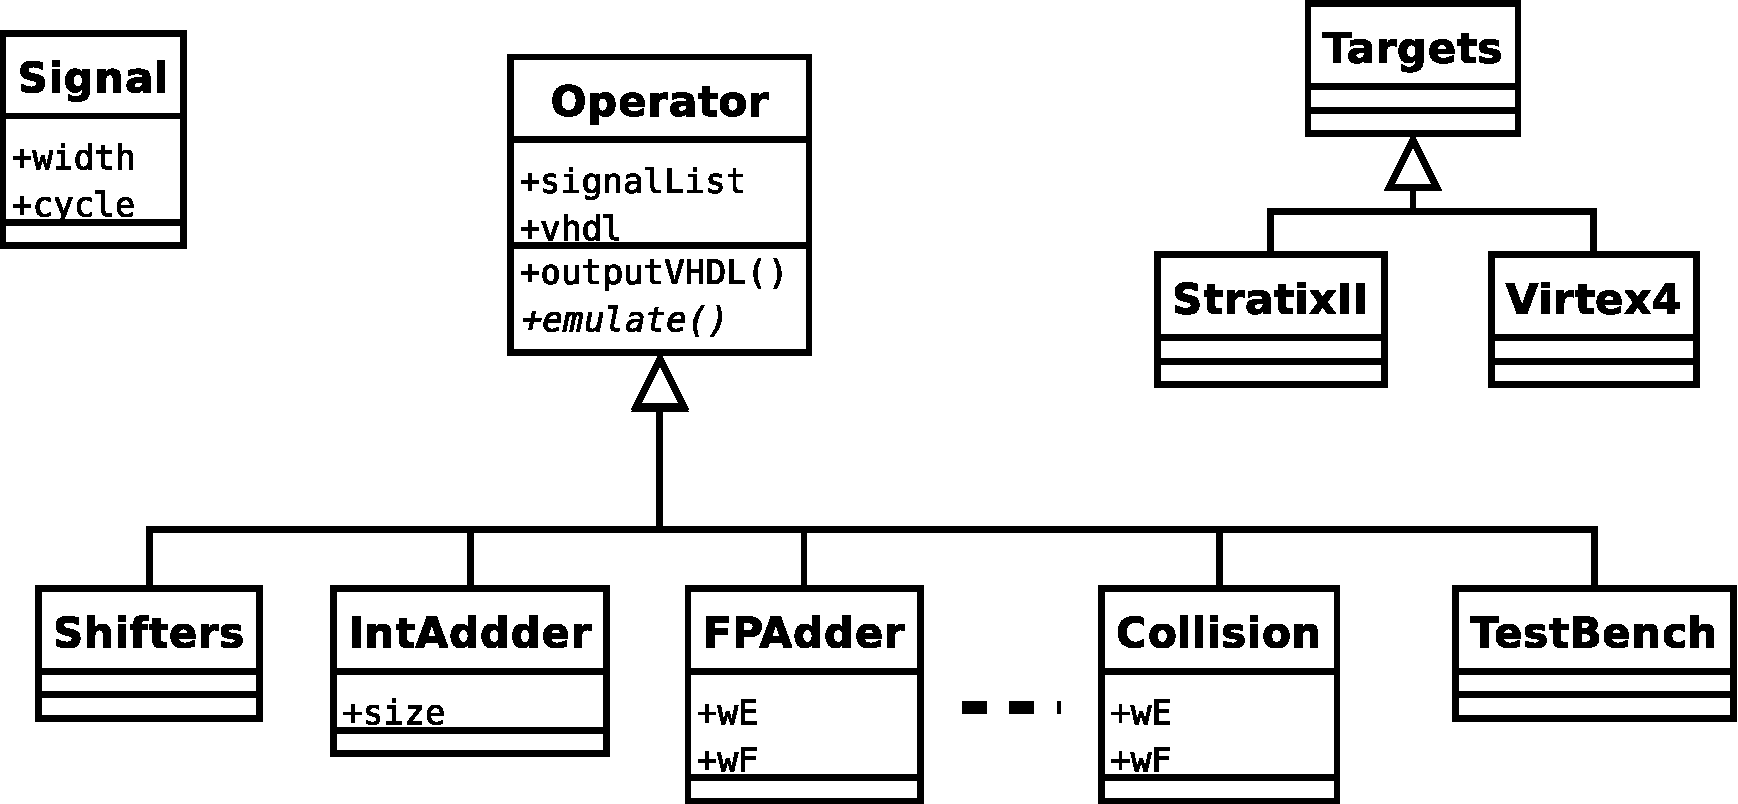
\includegraphics[width=0.7\textwidth]{../Figures/FloPoCoClasses.pdf}        
%  \end{latexonly}
\end{center}


\section{Data-types in FloPoCo\label{sec:data-types}}

\subsection{Floating-point numbers}

FloPoCo partly supports two floating-point formats: the standard IEEE-754 (generalized to arbitrary exponent and mantissa sizes), and its internal format (see the web documentation).
The internal format lacks subnormal support.
It also explicits the exceptional cases (zero, infinity, NaN) in two additional bits.
This makes it more hardware-efficient (no decoding/encoding of these exceptional cases in the exponent), but less memory-efficient.

\subsection{Fixed-point numbers}
In FloPoCo, a fixed point format is defined by a boolean true if signed, and two integers: the weights of the MSB and the LSB, which can be positive or negative. 
For instance the unit bit has weight 0, the point is between weights 0 and -1. 

These two weights are inclusive: The size of the corresponding bit vector will be MSB-LSB+1.
This is true for signed as well as unsigned numbers: If the format is signed, then the sign bit is the bit of weight MSB.


Now for a more stylistic, but nevertheless useful convention. Whenever an interface (be it to the command line, or to an internal function) includes the MSB and the LSB of the same format, they should appear in this order (MSB then LSB). This order corresponds to the order of the weights in the binary writing (the MSB is to the left of the LSB). 
When a boolean sign is passed as well, it should be first, for the same reason (the sign bit is the leftmost bit).

Examples:
\begin{itemize}
\item C char type corresponds to MSB=7, LSB=0.
\item a n-bit unsigned number between 0 and 1 has MSB=-1 and LSB=-n
\item a n-bit signed number between -1 and 1 has MSB=0 and LSB=-n+1
\end{itemize}

Finally, whenever we can live with integers, we should stick with integers and not obfuscate them as fixed-point numbers.




\section{Tutorial for new developers \label{sec:tutorial}}

The FloPoCo distribution include a dummy tutorial operator in \texttt{src/TutorialOperator.hpp} and \texttt{src/TutorialOperator.cpp}.
It describes an operator class \texttt{TutorialOperator} that you may freely modify without disturbing the rest of FloPoCo.

\texttt{TutorialOperator} is heavily documented, and this section assumes that you are looking at it.

After compiling FloPoCo, run in a terminal\\
\verb!./flopoco TutorialOperator!

You will obtain the documentation on the parameters of this operator.
This documentation is defined by the \texttt{TutorialOperator::registerFactory} method.

Now run in a terminal\\
\verb!./flopoco TutorialOperator param0=8 param1=8!

and you should obtain  some VHDL in \texttt{flopoco.vhdl}


\subsection{First steps in FloPoCo operator writing}

FloPoCo mostly requires you to embed the part of the VHDL that is between the \texttt{begin} and the \texttt{end} of the architecture
into the constructor of a class that inherits from
\verb!Operator!. The following is minimal FloPoCo code for
\verb!MAC.cpp!:
\begin{verbatim}
#include "Operator.hpp"

class MAC : public Operator
{
public:
// The constructor
MAC(Target* target): Operator(target)
{
	setName("MAC");
	setCopyrightString("ACME MAC Co, 2009");		

	// Set up the IO signals
	addInput ("X"  , 64);
	addInput ("Y"  , 32);
	addInput ("Z"  , 32);
	addOutput("R"  , 64);

   vhdl << declare("T", 64) << " <= Y * Z;" << endl;
   vhdl << "R <= X + T;" << endl;
}

// the destructor
	~MAC() {}
\end{verbatim}
 
And that's it. \verb!MAC! inherits from \verb!Operator! the method
\verb!outputVHDL()! that will assemble the information defined in the
constructor into synthesizable VHDL. Note that \verb!R! is declared by \verb!addOutput!.

So far we have gained little, except that is is more convenient to
have the declaration of \verb!T! where its value is defined. Let us
now turn this design into a pipelined one.

\subsection{Adding delay information}
A latency  may be passed as first optional argument to  \texttt{declare()}.
  This value decribes the contribution of this VHDL statement to the critical path.
  It is best defined using methods of \texttt{Target}.
  See \texttt{FPAddSinglePath} for examples.

\subsection{Sub-components: unique instances}

In FloPoCo, most instances are \emph{unique}: an \texttt{Operator} is built for a specific context, optimized for this context, and only one instance of this Operator will be used in the VHDL.
This is the default situation, because it allows the tool to optimize the pipelining of each component for its context.
The preferred method to use in such case is the \emph{newInstance()} method of Operator. 
See \texttt{FPAddSinglePath} for an example of a large component that instantiates many sub-components (several \texttt{IntAdder}, \texttt{Shifter}, etc).

\texttt{newInstance()} uses the factory-based user interface.
It is common to need a table of pre-computed values.
To get a unique instance of such a table,  first build the table content as a \verb!vector<mpz_class>!, then call \texttt{Table::newUniqueInstance()}.
See examples in \texttt{Trigs/FixSinCos.cpp}.


If for some reason you want to use a unique instance but don't want/need to expose a user interface for it, you just have to follow the same sequence of calls as you may find in \texttt{Table::newUniqueInstance()}.

Beware, the order is important for the operator scheduling to work properly, and it has changed since version 5.0.

\subsection{Sub-components: shared instances}

A component may also be shared (i.e. the same component is reused many times).
Simple examples are the tables in \texttt{FPConstDiv}, or in \texttt{IntConstDiv}.

The preferred method to use in such case is the \emph{newSharedInstance()} method of Operator, as in the following:
\begin{verbatim}
Operator* op = new MySubComponent(...);
op -> setShared();
//now some loop that creates many instances
for (....) {
  string myInstanceName = ...; 
  string actualX = ...;
  string actualR = ...;
  vhdl << declare(actualX, ..) << " <= " << ...;   
  newSharedInstance(op, myInstanceName, "X=>"+actualX, "R=>"+actualR);
}
\end{verbatim}

See \texttt{IntConstDiv} or \texttt{FPDiv} for detailed examples.

\subsection{Using the Table object}
Small tables of precomputed values are very powerful components, especially when targetting FPGAs.
They are quite often shared.

See \texttt{IntConstDiv} or \texttt{FPDiv} for examples of small, shared tables (intended to be implemented as LUTs on FPGAs, and as logic gates on ASIC).

See \texttt{FixFunctionByTable} for an example how to inherit \texttt{Table}.

See \texttt{FixFunctionByPiecewisePoly} for an example how to instanciate a \texttt{Table} as a sub-components.

TODO (not repaired yet): See \texttt{FPExp} for an example of unique Table intended to fit in a block RAM.


\section{Frequency-directed pipeline}

The  pipeline framework  is implemented mostly in the \texttt{Operator} and \texttt{Signal} classes, and we refer the reader to the source code for the full  details.
More details can also be found in \cite{istoan:hal-01373937}.

\subsection{VHDL generation for a simple component}

\subsubsection{First VHDL parsing and signal graph construction}
The \texttt{vhdl} stream is parsed (as the constructor writes to it) to locate VHDL signal identifiers.

This pass builds  a signal graph, an example of which is shown on Figure~\ref{fig:depgraphShifter} 
(it was obtained in \texttt{flopoco.dot} by the command
\verb!./flopoco Shifter wIn=8 maxshift=8 dir=1! )

In this graph, the nodes are signals (of the FloPoCo \texttt{Signal} class), and the edges are signal dependencies, \emph{i.e.} which signal is computed out of which signal.
Technically, the graph is built by defining predecessors and successors of each \texttt{Signal}.

The operations between the signals are not kept in this graph: they are kept in the \texttt{vhdl} stream.
  However, their latency (passed as first optional argument to  \texttt{declare()}) is used to label each signal.
  This value decribes the contribution of this VHDL statement to the critical path.

  In Figure~\ref{fig:depgraphShifter}, the first line of each box is the signal name.
The second line is the critical path contribution of each signal.
  The third line is the actual global timing of each signal, which is computed in the following. 
  
The reader interested in this first parsing pass should have a look at \texttt{FlopocoStream.cpp}.

  \begin{figure}
    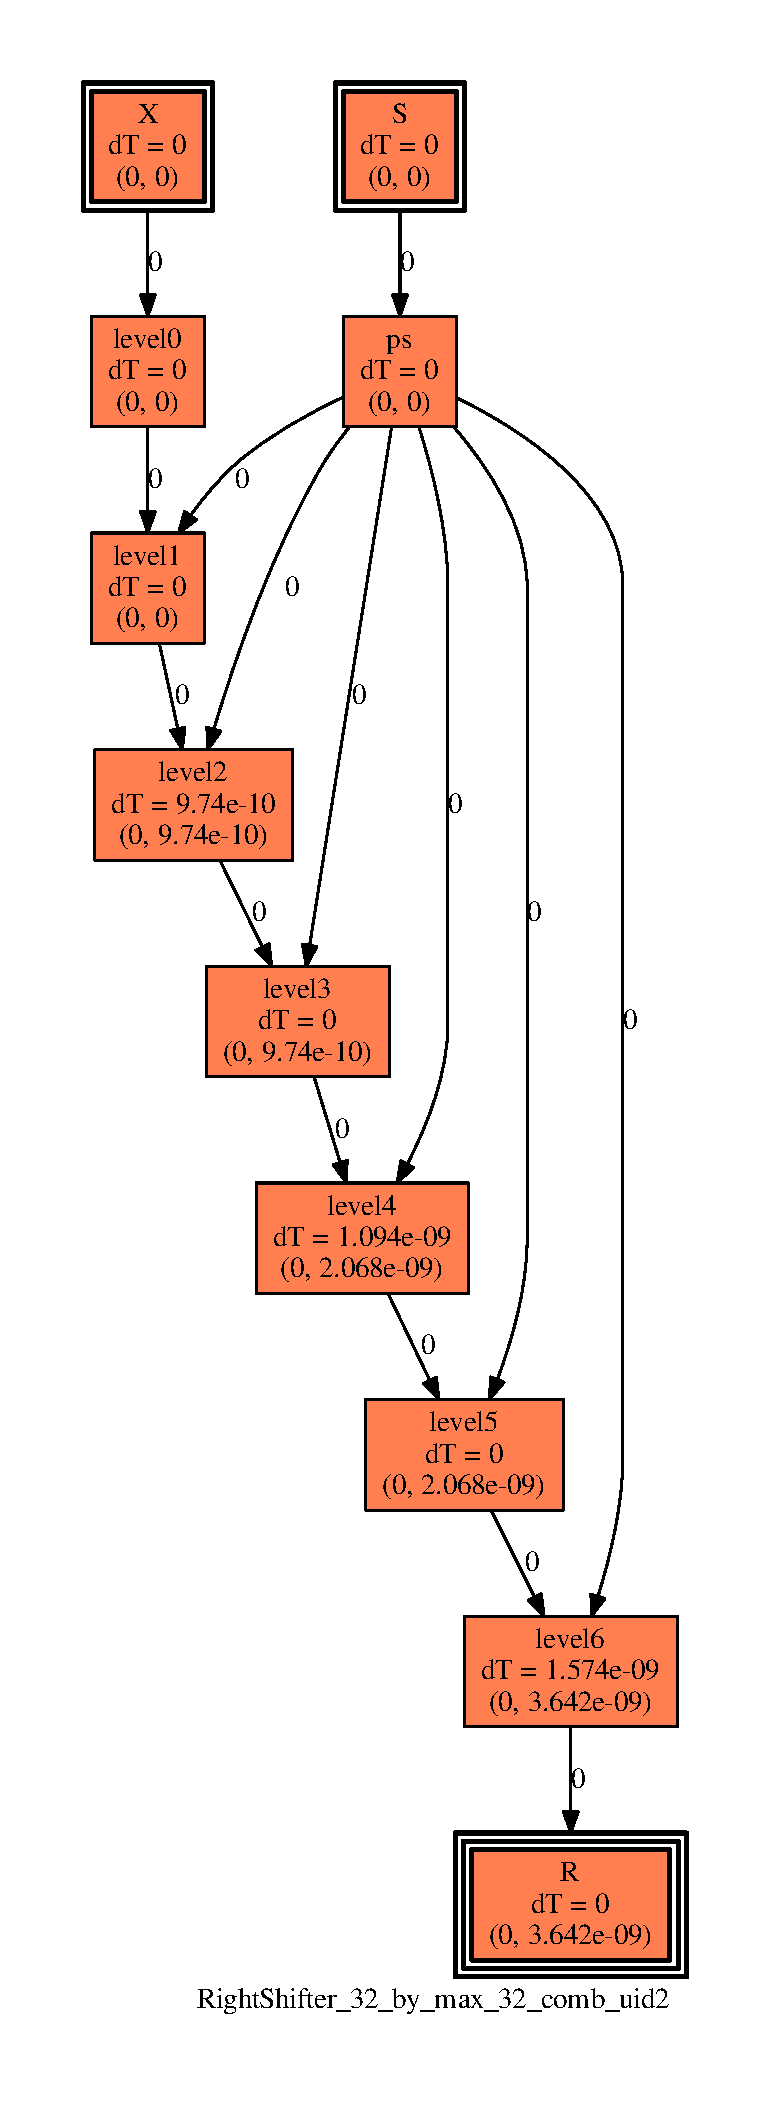
\includegraphics[width=0.4\textwidth]{Fig/depgraphShifterNoPipe}
    \hfill
    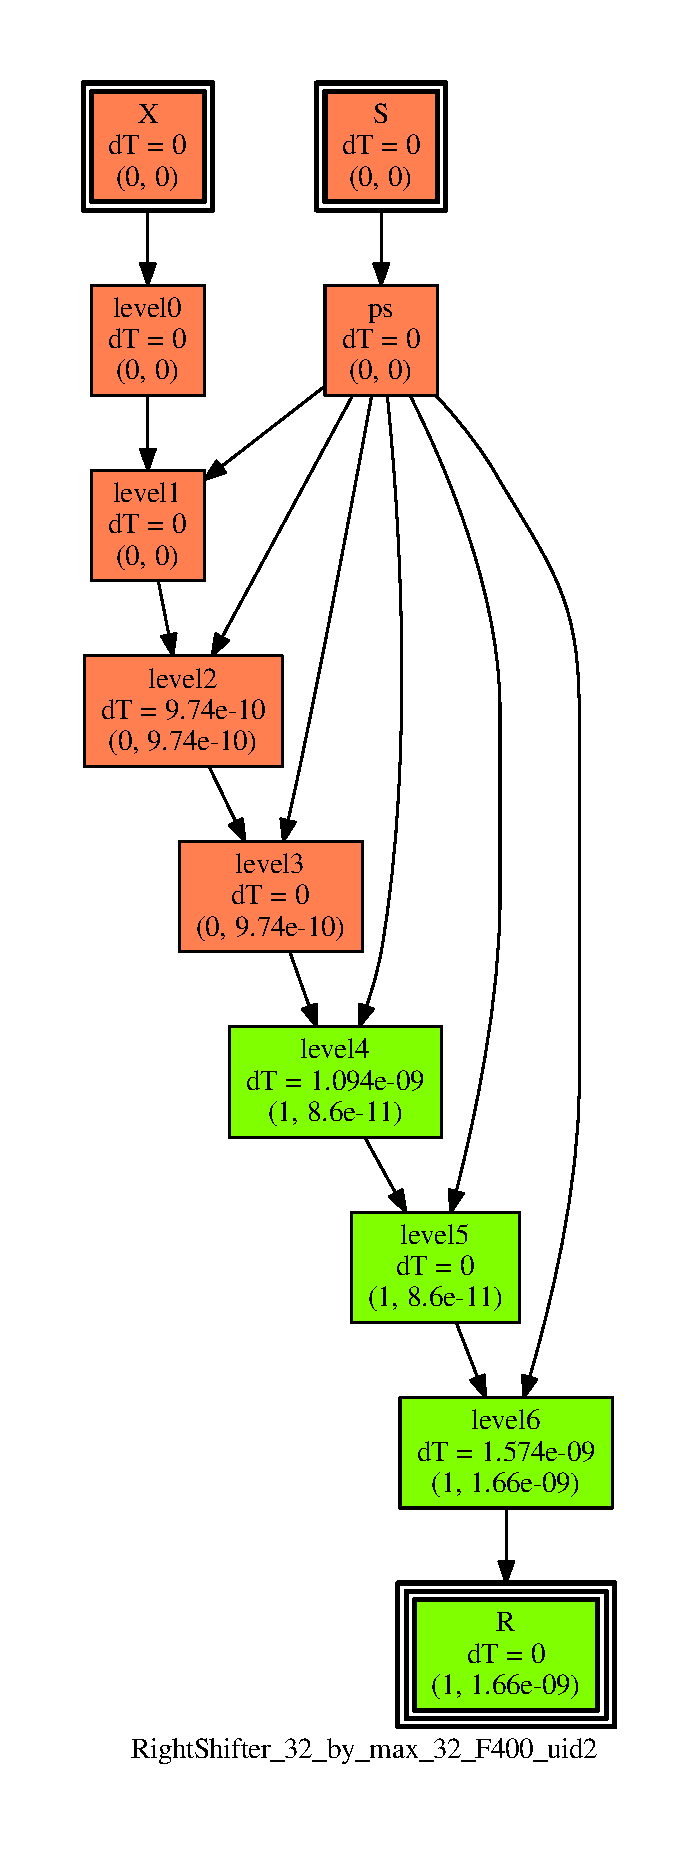
\includegraphics[width=0.4\textwidth]{Fig/depgraphShifterPipelined}
		\centering
		\caption{S-Graph for a combinatorial 8-bit barrel shifter, combinatorial (left) and pipelined (right)}
		\label{fig:depgraphShifter}
	\end{figure}    


\subsubsection{Scheduling of the signal graph}\label{sec:scheduling}
The second step of automatic pipelining is the scheduling of the signal graph.
It is implemented in the method \texttt{Operator::schedule()}.
It is an ASAP (as soon as possible) scheduling: starting from the input, we accumulate the critical path along the edges of the signal graph.

With the \texttt{pipeline=no} option, what we obtain in \texttt{flopoco.dot} is an estimate of the critical path from an input to each signal.


With \texttt{pipeline=yes}, the schedule constructs a pipeline.
Each signal is assigned a cycle and a critical path within this cycle (i.e. what we obtain in \texttt{flopoco.dot} is an estimate of the critical path from the output of a register to each signal.

The timing of a signal is therefore expressed as a pair $(c, \tau)$, where
\begin{itemize}
\item $c$ is an integer that counts the number of registers
  on the longest path from an input to $s$.
\item $\tau$ is a real number that represents the critical path delay (in seconds)
  from the last register or earliest input to $s$.
\end{itemize}

The colors on Fig. \ref{fig:depgraphShifter}, right,  indicate the cycle.
The complete lexicographic time of each signal is given by the third line of each signal box. 

There is a lexicographic order on such timings: $(c_1, \tau_1) > (c_2, \tau_2)$ if $c_1 > c_2$ or if $c_1 = c_2$ and $\tau_1 > \tau_2$.

\subsubsection{Back-annotation of the VHDL stream with delay information}
Once each signal is scheduled, there is a second parsing step of the VHDL stream that delays each signal where it is needed by the proper number of cycle.
Technically, when parsing
\verb!A <= B and C;!, the schedule has ensured that  \verb!B.cycle!$\le$ \verb!A.cycle!.
If \verb!A.cycle! $>$ \verb!B.cycle!, FloPoCo delays
signal \verb!B! by n=\verb!A.cycle! $-$ \verb!B.cycle! cycles.

Technically, it just replaces, in the output VHDL,   \verb!B! with \verb!B_dn!.
It also updates bookkeeping information that gives the life span of each signal.

This process is performed by the \verb!Operator::applySchedule()! method.

\subsubsection{Final VHDL output}
The final step adds to the VHDL stream constructed from previous step all the declarations (entities, signals, etc) as well as the shift registers that delay signals.
It is performed by the \verb!Operator::outputVHDL()! method.

\subsection{Subcomponents and instance}

Now consider the more complex situation of a component that include other subcomponents.
There are two distinct situations:
\begin{itemize}
\item either the subcomponent is used only once, in which case we want to schedule it in its context.
  This is the default situation.
  An extensive example of a complex component built by assembling simpler ones is \texttt{FPAddSub/FPAddSinglePath}.
  
\item Or, the subcomponent is used many times (a typical example is the compressor in a bit heap), in which case all the instances will necessarily share the same schedule.
  In FloPoCo, we add a constraint in this case: such operators remain very small and thus shall not be pipelined.
  This covers 100\% of the use cases so far.
  Such components have to be declared shared by calling \texttt{Operator::setShared()}.
\end{itemize}

In the following we detail these two cases and what happens under the hood in terms of scheduling.


\subsubsection{Unique instances}
In this case, the entity of the subcomponent is used in only one VHDL instance.

FloPoCo provides for this case a single method, \verb!Operator::newInstance()!.
Its inputs are those provided on the command-line interface, therefore this method will only work for operators which implement the factory methods.
It returns a pointer to the newly created \texttt{Operator}.

In terms of VHDL, \verb!Operator::newInstance()! creates both the entity of the subcomponent (by calling its constructor) and an instance of this entity in the \texttt{vhdl} stream of the current buffer.

Let us now see what happens in terms of scheduling and pipelining.
\begin{itemize}
\item In the signal graph, \verb!Operator::newInstance()! connects the actual signals to the subcomponent ports, with simple wires (no delay added to the critical path).
  The \texttt{flopoco.dot} output shows a box around the signals of the subcomponent, but there is one single graph linking \texttt{Signal} objects.

\item It is useful that the constructor of the subcomponent may take decisions based on the schedule of its inputs (example: the \texttt{IntAdder} pipelined integer splits its inputs depending on their critical path).
  Therefore, \verb!Operator::newInstance()! calls \verb!Operator::schedule()! (step \ref{sec:scheduling} above).

  Since there is only one big signal graph, \verb!Operator::schedule()! first gets to the root of the component hierarchy, before actually computing the schedule, starting from the inputs of this root.

\item When the inputs to a sub-component are not synchronized, they will be synchronized inside the sub-component.

\item It is important to understand that \verb!Operator::schedule()! can be invoked on an incomplete graph.
  In such an ASAP scheduling, the schedule of a signal is only defined by the schedule of its predecessors: once it is computed, it will no longer change, so \verb!Operator::schedule()! may be called several times. It will be called by default after the end of the constructor of a root operator (so the signal graph is complete).

\item All this probably works best (only works?) if the VHDL is written in the natural order, from inputs to outputs... 

\end{itemize}


  \begin{figure}
    
\includegraphics[height=\textheight]{Fig/depgraphFPAddPipelined}
		\centering
		\caption{S-Graph for a pipelined FPAddSinglePath operator. Zoom on the Shifter component and observe that it has been pipelined for its context.}
		\label{fig:depgraphFPAdd}
	\end{figure}    



\subsubsection{Shared instances}

Again, shared instances are small, purely combinatorial components.

Here are the main differences:
\begin{enumerate}
\item The constructor of the subcomponent must be called only once.
\item The instances themselves must be somehow replicated in the signal graph.
\end{enumerate}
The solution chosen is to replace \emph{in the signal graph} instances with links between the inputs and outputs.
Each output is labeled with a critical path contribution,   equal to the critical path of this output in the instance.

This is performed under the hood by the \verb!Operator::inPortMap()!, \verb!Operator::outPortMap()! and \verb!Operator::instance()! methods.

An instance is combinatorial, hence lives within a single cycle.
Therefore, all the outputs of a shared instance have this same cycle.
All the inputs are also input at this same cycle to the instance (they are delayed in the \texttt{port map}.
If a pipeline register is inserted to account for the delay of a shared instance, it is inserted on the outputs.

The simplest example of shared instances is currently \texttt{FPDivSqrt/FPDiv}.


\section{Test bench generation}\label{sec:test-bench-gener}

\subsection{Overview}
\texttt{\small Operator} provides one more virtual method, \texttt{\small emulate()},
to be overloaded by each Operator. As the name indicates, this method
provides a bit-accurate simulation of the operator.
 
Once this method is available, the command\\
 \texttt{flopoco FPAdd we=8 wf=23 TestBench n=500} \\
produces a test bench of 500 test vectors to exercise \texttt{\small FPAdd}. 

This test bench is properly synchronized if the operator under test happens to be pipelined: \texttt{\small emulate()} only has to specify the mathematical (combinatorial) functionality of the operator.

The \texttt{\small emulate()} method should be considered  the specification of the behaviour of the operator.
Therefore, as any instructor will tell you, it should be written \emph{before} the code generating the VHDL of the operator (test-driven design).


To see examples of \texttt{emulate()} functions, see
\begin{itemize}
\item \texttt{IntAdder} or \texttt{IntConstDiv} for an operator with integer inputs and outputs;
  For these, the GNU Multiple Precision library is your friend.
\item \texttt{FixRealKCM} for an operator with fixed-point inputs and outputs;
\item \texttt{FPAdd}  for an operator with floating-point inputs and outputs;
  For these, your friend is the GNU MPFR library, and FloPoCo provides all the needed helper functions to convert between bit vectors and MPFR numbers.
\end{itemize}


\subsection{\texttt{emulate()}  internals}
\texttt{\small emulate()} has a single argument which is a \texttt{\small TestCase}.
This is a data-structure associating inputs to outputs.
Upon entering \texttt{\small emulate()}, the input part is filled (probably by \texttt{\small TestBench}), and the purpose of \texttt{\small emulate()} is to fill the output part.
\texttt{\small emulate()} is completely generic:
Both inputs and outputs are specified as bit vectors.
However these vectors are stored for convenience in \texttt{\small mpz\_class} numbers.
This class is a very convenient C++ wrapper around GMP, which can almost be used as an \texttt{\small int}, but without any overflow issue.

Therefore an input/output is a map of the name (which should match those defined by \texttt{\small addInput} etc.) and a \texttt{\small mpz\_class}.
When the input/outputs are integers, this is a perfect match.

When the input/outputs are floating-point numbers, the most convenient multiple-precision library is MPFR.
However the I/Os  are nevertheless encoded as \texttt{\small mpz\_class}.
The \texttt{\small emulate()} method therefore typically must
\begin{itemize}
\item convert the \texttt{\small mpz\_class} inputs to arbitrary precision floating-point numbers in the MPFR format -- this is done with the help of the \texttt{\small FPNumber} class;
\item compute the expected results, using functions from the MPFR library;
\item convert the resulting MPFR number into its bit vector, encoded in an \texttt{\small mpz\_class}, before completing the \texttt{\small TestCase}. 
\end{itemize}
This double conversion is a bit cumbersome, but may be copy-pasted from one existing operator: Imitate \texttt{\small FPAddSinglePath} or \texttt{\small FPExp}.


\subsection{Fully and weakly specified operators}
 Most operators should be fully specified: for a given input
  vector, they must output a uniquely defined vector. This is the case of 
  \texttt{\small IntAdder} above. For floating-point
  operators, this unique output is the combination of a mathematical
  function and a well-defined rounding mode. The bit-exact MPFR
  library is used in this case. Imitate \texttt{\small FPAddSinglePath} in this case.

 Other operators are not defined so strictly, and may have  several acceptable output values.
 The last parameter of \texttt{\small addOutput} defines how many values this output may take.
 An common requirement is \emph{faithful rounding}: the operator should return one of the two FP values surrounding the exact result\footnote{
 The allowed error is twice as large as correct rounding, so a correctly rounded result on $p$ bits is as accurate as a faithful result on $p+1$ bits. 
 However, (for reasons too long to detail here) a faithful operator may be much, much cheaper to build than a correctly rounded one.
 In such cases it is cheaper to build a faithful operator to $p+1$ bits than a correctly rounded one to precision $p$.}
These values may be obtained thanks to the  \emph{rounding up} and \emph{rounding down} modes supported by MPFR.
See \texttt{\small FPExp} or \texttt{\small FPLog} for  examples in floating point, and \texttt{FixSinCos} for an example in fixed point (which is also an example where the function has two outputs).

\subsection{Operator-specific test  vector generation}
Overloading \texttt{\small emulate()} is enough for FloPoCo to be able
to create a generic test bench using random inputs. The default random generator is uniform over the input bit vectors. It is
often possible to perform better, more operator-specific test-case
generation. Let us just take two examples.

\begin{itemize}\item 
  A double-precision exponential returns $+\infty$ for all inputs
  larger than 710 and returns $0$ for all inputs smaller than
  $-746$. In other terms, the most interesting test domain for this
  function is when the input exponent is between $-10$ and $10$, a
  fraction of the full double-precision exponent domain ($-1024$ to
  $1023$). Generating uniform random 64-bit integers and using them as
  floating-point inputs would mean testing mostly the
  overflow/underflow logic, which is a tiny part of the operator.


\item In a floating-point adder, if the difference between the
  exponents of the two operands is large, the adder will simply return
  the biggest of the two, and again this is the most probable
  situation when taking two random operands. Here it is better to
  generate random cases where the two operands have close
  exponents. Besides, a big part of the adder architecture is
  dedicated to the case when both exponents differ only by 1, and
  random tests should be focused on this situation.
\end{itemize}
Such cases are managed by overloading the Operator method  \texttt{\small buildRandomTestCases()}. 
See \texttt{FPExp.cpp} and \texttt{FPAdd.cpp} for the examples above.

\subsection{Corner-cases and regression tests}
Finally, \texttt{\small buildStandardTestCases()} allows to test corner cases which random testing has little chance to find.
See \texttt{\small FPAdd.cpp} for examples. 

Here, it is often useful to add a comment to a test case using \texttt{\small addComment}: these comments
will show up in the VHDL generated by \texttt{\small TestBench file=false}.


\section{Regression testing, build test }
The command \verb!flopoco Autotest Operator=FPadd! tests FPAdd for a range of relevant parameter values.
For each parameter vector, it reports if the FloPoCo command succeeded, if the VHDL was syntactically correct, and if the simulation of this VHDL was successful.

The enumeration of the parameter vectors is defined in the (optional) static method \texttt{FPAdd::unitTest()}.
This is a relatively recent addition to the framework, and not all operators support it, but it is strongly advised to set it up in the early steps of operator development: it helps uncover bugs that occur for specific values of the parameters.

The command \verb!flopoco Autotest Operator=all! runs this test for all the operators that support it.
It may take long...

\section{Bit heaps}

The main interface to the developer is the  \texttt{BitHeap} class, which encapsulates all the needed data structures and methods. 
The bits to be added to a \texttt{BitHeap} are simply  signals of the operator being generated.
This makes it possible to define the initial bit heap, which can be of any shape or size. 
The \texttt{BitHeap} class also implements the compressor tree optimization techniques presented in \cite{DinIstSer2013-FPL-BitHeap,kz14a,kz14b,kk18} (the compression algorithm is selected on the command line), and can generate the corresponding hardware.


%dynamical data structure that evolves during the circuit generation process.

The typical code to generate the architecture of an operator involving a bit heap is shown in Listing~\ref{algo:code-bitheap}.
The main methods to manipulate the bit heap are shown in Table~\ref{tab:bit_heap_interface}.
Basically, there is everything to add or subtract single bits, signed or unsigned numbers held in bit vectors, or constants. 
Once all the bits have been thrown on the bit heap, the \texttt{startCompression()} method launches the optimization of the compressor tree as well as the VHDL code generation.


\lstset{language=C++,numbers=none,basicstyle=\small\ttfamily,xleftmargin=5pt,xrightmargin=0pt,frame=lines,rulesepcolor=\color{black},keywordstyle=\color{black}\bfseries,escapeinside={(*}{*)},belowskip=-10pt}

\begin{lstlisting}[float, caption=Typical code for an operator involving a bit heap, label=algo:code-bitheap]
bh = new BitHeap(...);  // create an empty bit heap

// construction of the bit heap
for (...) {
  // generate VHDL that defines signals such as
  ///  mySingleBit or myBitVector
  ...
  
  // then add these signals to the bit heap: 
  bh->addBit(myBit, pos1); // no VHDL generation here 
  bh->addSignal(mybitVector, pos2); // nor here
}

// generate the compressor tree for the bit heap
bh->startCompression(); // this line generates a lot of VHDL
\end{lstlisting}


Some operators that use the BitHeap have two constructors:
\begin{itemize}
	\item one standalone, classical; The BitHeap is constructed in the operator and used only for this operator
	\item one virtual; a BitHeap from another operator is provided that is shared among the operators (which can build a more complex operator).
\end{itemize}

In the latter case, the typical arithmetic flow requires to first perform some error analysis to determine a number of guard bits to add to the bit heap.
This must be done before any VHDL generation.
If we want to delegate some of this error analysis to the subcomponents, then either it must be implemented in some static method of the Operator, or the constructor must delay the actual VHDL output to another method.

For an example of this in practice, see \texttt{FixFilters/FixSOPC}.

\begin{table}[t]
  \centering
    \begin{center}
      \caption{The main methods of the \texttt{BitHeap} interface}
	\label{tab:bit_heap_interface}
  \footnotesize
  
    \begin{tabular}{L{0.5\textwidth}L{0.4\textwidth}}
    	\toprule
		Method                                        & Description                                      \\
    	\midrule
      {\texttt{void addBit(string sigName,int pos)}}      & Add a single bit                                 \\
      {\texttt{void addSignal(string sigName,int shift)}}   & Add a fixed-point signal, with sign extension if needed                       \\
      {\texttt{void subtractSignal(string name,int shift)}} & Subtract a fixed-point signal, with sign extension if needed                  \\
      {\texttt{void addConstantOneBit(int pos)}}  & Add a constant one bit                           \\[1ex]
      {\texttt{void addConstant(mpz\_class cst,int pos)}} & Add the constant $\mathtt{cst}\cdot 2^{\mathtt{pos}}$ \\
      {\texttt{void startCompression()}}          & Generate a compressor tree                       \\
    	\bottomrule
    \end{tabular}
        When the argument is a signal name, it is used to refer to a FloPoCo object of the class Signal, which encapsulate a fixed-point format with its  signedness, its MSB, and its LSB.
    \end{center}
\end{table}



\subsection{The data structure}
This section and the following describe the internals of the \texttt{BitHeap} class, and are intended for developers wishing to extend the BitHeap framework itself (e.\,g., with new compressors or compression algorithms).

A \emph{weighted bit} is a data structure consisting essentially of a signal name, a bit position, and various fields used when building the compressor tree.
In FloPoCo the \texttt{Signal} class also encapsulates the timing of each signal, so each weighted bit also carries its arrival time.


A column of the bit heap is represented as a list of weighted bits.
This list is  sorted by the  arrival time of the bits, so that compression algorithms can compress first the bits arrived first.

The complete bit heap data structure essentially consists of its MSB and LSB, and an array of columns indexed by the positions. 

The \texttt{BitHeap} class also offers methods to visualize a bit heap as a dot diagram like the one shown in Figure~\ref{fig:bitheapgallery-halfsine}.
Use the \texttt{generateFigures} flag to enable the output of \texttt{SVG} and \texttt{.tex} files (these use the macros found in \texttt{dot\_diag\_macros.tex}).
Different arrival times may be indicated by different colors.

FloPoCo may generate such figures as SVG files that can be opened in a browser, in which case hovering the mouse over one bit shows its signal name and its arrival instant in circuit time.  
%Bits are inserted in the bit heap at the proper instant in the circuit time. This evolution of the bit heap in  should not be confused with the evolution of the bit heap in the circuit time. 

%It should be clear that there are two aspects of time here: operator-generation time (as the generator program runs), and circuit time (using notions such as critical path or, for pipelined designs, cycles). 
%The generator must be able to evaluate the circuit time, for instance as in \cite{DinechinPasca2011-DaT}.

\begin{figure}[t]
  \centering
    % obtained directly from FloPoCo
    % $ ./flopoco FixHalfSine lsbIn=-16 lsbout=-16 n=4
    \scalebox{0.28} {
      \begin{dotdiag}{20}
        \begin{scope}
          \drawdotcol{0}{16}
          \drawdotcol{1}{16}
          \drawdotcol{2}{16}
          \drawdotcol{3}{16}
          \drawdotcol{4}{14}
          \drawdotcol{5}{12}
          \drawdotcol{6}{12}
          \drawdotcol{7}{12}
          \drawdotcol{8}{12}
          \drawdotcol{9}{10}
          \drawdotcol{10}{8}
          \drawdotcol{11}{8}
          \drawdotcol{12}{8}
          \drawdotcol{13}{8}
          \drawdotcol{14}{6}
          \drawdotcol{15}{4}
          \drawdotcol{16}{4}
          \drawdotcol{17}{4}
          \drawdotcol{18}{4}
          \drawdotcol{19}{3}
        \end{scope}
      \end{dotdiag}
    }
  \caption{Bit heap obtained for a 16-bit, 8-tap half-sine pulse shaping FIR filter operator \texttt{FixHalfSine}}
  \label{fig:bitheapgallery-halfsine}
\end{figure}

\subsection{Compressor tree generation}

Once the data structure of the BitHeap is created by using the methods of Table~\ref{tab:bit_heap_interface}, the compressor tree generation is started by calling \texttt{startCompression()}.
It involves the following steps:
\begin{enumerate}
	\item The algorithm for solving the compressor tree problem is selected (a derived class from \texttt{CompressionStrategy}).
	\item A list of possible (target-dependent) compressors is generated (class \texttt{BasicCompressor} for representing the shape and class \texttt{Compressor} implementing the Operator performing the compression).
	\item Then, the bits of the bit heap are scheduled to different stages according to their cycle and combinatorial arrival time.
	\item Next, the compressor trees are optimized (by a class derived from \texttt{CompressionStrategy}) and a \texttt{BitHeapSolution} object is created. This solution contains the used compressors per stage and column.
	\item Finally, the VHDL code of the compressor tree is generated.
\end{enumerate}

New compressor tree optimization methods can be implemented  by extending \texttt{CompressionStrategy}.



\section{Writing a new target}
Try to fill data such as LUT input size (\texttt{lutInputs()}), etc.

Here are some operators that can be used to calibrate delay functions.
You may use the scripts in \texttt{tools/} to launch syntheses and get critical path reports.
It is better to ask for a relatively low frequency (say, half peak, 200MHz) to avoid troubles with I/O buffer delays when using post place-and-route synthesis.

\begin{itemize}
\item To calibrate the logic delay, use 
\begin{verbatim}
  ./flopoco IntConstDiv wIn=64 d=3 Wrapper
\end{verbatim}
  If you have specified your lutInputs properly, the architecture should be a sequence of LUTs connected by local routing.
  First check that the estimated cost reported by FloPoCo matches the actual cost. 
  
\item To calibrate the IntAdder delay, use
\begin{verbatim}
  ./flopoco IntAdder wIn=64 Wrapper
\end{verbatim}
  for increasing values of 64.
  
\end{itemize}


\bibliographystyle{IEEEtran}
% argument is your BibTeX string definitions and bibliography database(s)
\bibliography{../web/bib/flopoco.bib,../web/bib/flopoco-users.bib}

\end{document}
